%Copyright 2014 Jean-Philippe Eisenbarth
%This program is free software: you can 
%redistribute it and/or modify it under the terms of the GNU General Public 
%License as published by the Free Software Foundation, either version 3 of the 
%License, or (at your option) any later version.
%This program is distributed in the hope that it will be useful,but WITHOUT ANY 
%WARRANTY; without even the implied warranty of MERCHANTABILITY or FITNESS FOR A 
%PARTICULAR PURPOSE. See the GNU General Public License for more details.
%You should have received a copy of the GNU General Public License along with 
%this program.  If not, see <http://www.gnu.org/licenses/>.

%Based on the code of Yiannis Lazarides
%http://tex.stackexchange.com/questions/42602/software-requirements-specification-with-latex
%http://tex.stackexchange.com/users/963/yiannis-lazarides
%Also based on the template of Karl E. Wiegers
%http://www.se.rit.edu/~emad/teaching/slides/srs_template_sep14.pdf
%http://karlwiegers.com
\documentclass{scrreprt}
\usepackage{tikz}
\usepackage{listings}
\usepackage{underscore}
\usepackage[bookmarks=true]{hyperref}
\usepackage[utf8]{inputenc}
\usepackage[english]{babel}
\usepackage{pgfgantt}
\usepackage{CJKutf8}
\hypersetup{
    bookmarks=false,    % show bookmarks bar?
    pdftitle={Software Requirement Specification},    % title
    pdfauthor={Jean-Philippe Eisenbarth},                     % author
    pdfsubject={TeX and LaTeX},                        % subject of the document
    pdfkeywords={TeX, LaTeX, graphics, images}, % list of keywords
    colorlinks=true,       % false: boxed links; true: colored links
    linkcolor=blue,       % color of internal links
    citecolor=black,       % color of links to bibliography
    filecolor=black,        % color of file links
    urlcolor=purple,        % color of external links
    linktoc=page            % only page is linked
}%
\def\myversion{1.0 }
\date{}
%\title
\usepackage{hyperref}
\begin{document}
\begin{CJK}{UTF8}{bkai}
\begin{center}
    \begin{bfseries}
        \Huge{開放平台\\期末報告}\\
        \vspace{3.8cm}
        $<$柯B$>$\\
        \vspace{1.9cm}
        \LARGE{成員:}\\
        \vspace{1.0cm}
        范喻成\\
        \vspace{0.5cm}
        陳識允\\
        \vspace{0.5cm}
        黃柏凱\\
        \vspace{0.5cm}
        張哲家\\
        \vspace{0.5cm}
        \today\\
    \end{bfseries}
\end{center}

\tableofcontents

\chapter*{Revision History}

\begin{center}
    \begin{tabular}{|c|c|c|c|}
        \hline
	    Name & Date & Reason For Changes & Version\\
        \hline        
	    哲家 & 2018/6/15 & 把heroku上面的資料連結到github & 1\\
        \hline        
	    柏凱 & 2018/6/15 & 新增查詢電影的功能加入 & 2\\
        \hline
	    柏凱 & 2018/6/15 & 修復查詢電影的bug & 3\\
        \hline
	    柏凱 & 2018/6/15 & 新增requirements.txt的需求軟件 & 4\\
        \hline
	    識允 & 2018/6/15 & 新增youtube功能 & 5\\
        \hline
	    喻成 & 2018/6/15 & 新增latex和基本介紹 & 6\\
        \hline
	    哲家 & 2018/6/16 & 排版 & 7\\
        \hline
	    哲家 & 2018/6/17 & 新增翻譯功能 & 8\\
        \hline
	    哲家 & 2018/6/18 & 翻譯debug & 9\\
        \hline
	    識允 & 2018/6/18 & 更新youtube功能和新增help & 10\\
        \hline
	    哲家 & 2018/6/18 & bug fixed & 11\\
        \hline
	    哲家 & 2018/6/19 & 新增portal查詢作業與查氣象功能 & 12\\
        \hline
	    哲家 & 2018/6/19 & 修改requirements bug & 13\\
        \hline
	    識允 & 2018/6/19 & 修改氣象和翻譯 & 14\\
        \hline
	    哲家 & 2018/6/19 & portal改良 & 15\\
        \hline
	    哲家 & 2018/6/19 & bug fixed & 16\\
        \hline
	    哲家 & 2018/6/20 & portal防呆 & 17\\
        \hline
	    喻成 & 2018/6/20 & 更新latex & 18\\
        \hline
	    柏凱 & 2018/6/20 & 新增latex_ppt & 19\\
        \hline
	    識允 & 2018/6/20 & latex_ppt新增background & 20\\
        \hline
	    哲家 & 2018/6/21 & bug fixed & 21\\
        \hline
	    柏凱 & 2018/6/21 & 新增latex_ppt的設計理念與語意分析介面 & 22\\
        \hline
	    喻成 & 2018/6/21 & 修正latex & 23\\
        \hline
	    喻成 & 2018/6/21 & latex新增圖片 & 24\\
        \hline
	    識允 & 2018/6/21 & 新增latex的commit版本 & 25\\
        \hline
    \end{tabular}
\end{center}

\chapter{作品大綱}

這次要做的是之前在Line風行一時的LineBot,就是根據特定的話語,它會有不同的反應,所以我們試著利用py來做出也能在Line上運行的機器人,它的功能有{\color{red}最新電影建議}、{\color{red}新聞}、{\color{red}隨機一張狗狗貼圖}、{\color{red}天氣查詢}、{\color{red}Youtube影片查詢}、{\color{red}中英翻譯}、{\color{red}portal作業查詢},詳細功能會在下方解說。

\begin{center}
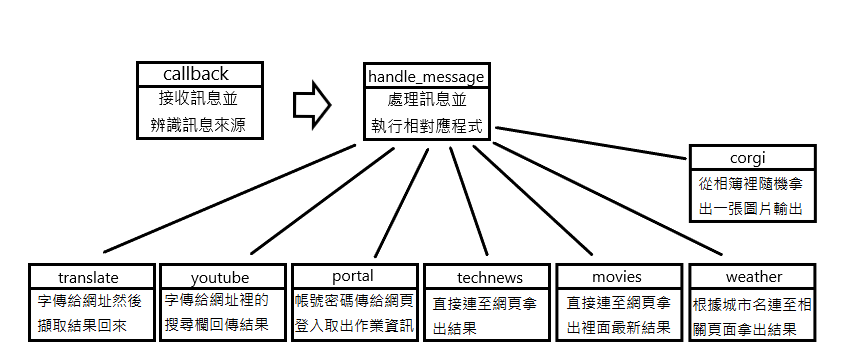
\includegraphics[width=15cm,height=6.5cm]{flow.png}
\\流程圖
\end{center}

\chapter{功能}

\section{最新電影建議}

只要打出{\color{red}moive},我們的機器人就會幫你找出目前最新的電影提共給你參考,不用怕想不到有甚麼電影好看!

\section{隨機呼叫狗狗圖片}

如果你打了{\color{red}狗狗}二字,我們的機器人就會po給你可愛的狗狗圖片,好慰藉你的心!

\section{YouTube搜尋}

聊天的時候剛好想到某一首歌或者一部影片,但是覺得開啟Youtube再按分享太耗時間了嗎? 沒關西!只要打上{\color{red}youtube 你想要查的名字},它就會幫你找到囉!

\section{新聞清單}

想找點時事來看,卻又不知道從何找起嗎? 只要打上{\color{red}news},機器人就會為您服務!

\section{中英翻譯}

想要說出一些英文? 或是想要迅速知道這個英文的意思? 打上{\color{red}翻譯 你要翻譯的字},不管是中翻英,還是英翻中,都是輕輕鬆鬆的拉!

\section{portal作業查詢}

想要迅速找到作業的狀況(僅限元智大學),別擔心,只要打上{\color{red}portal 帳號 密碼},就會顯示給你看嚕!

\section{天氣查詢}

想要知道今天究竟有怎麼樣的天氣嗎? 大聲呼叫{\color{red}天氣 城市名},就會出現拉!

\section{指令查詢}

忘記怎麼利用機器人了嗎!沒關西只要呼叫{\color{red}HELP},它就會告訴你指令怎麼用囉!

\chapter{Reference}

news$:$ {\color{blue}https://technews.tw/}\\
translate$:$ {\color{blue}http://translate.google.com/}\\
movie$:$ {\color{blue}https://movies.yahoo.com.tw/}\\
Youtube$:$ {\color{blue}https://www.youtube.com/}\\
weather$:$ {\color{blue}https://www.cwb.gov.tw/}\\
portal$:$ {\color{blue}https://portalx.yzu.edu.tw/}

\end{CJK}
\end{document}
